\documentclass[11pt]{article}
\usepackage[utf8]{inputenc}
\usepackage{microtype}
\usepackage{setspace}
\usepackage{listings,verbatim}
\usepackage{float}
\usepackage{algpseudocode,algorithm}
\usepackage[a4paper, total={6in, 9in}]{geometry}
\usepackage{graphicx} % Required for inserting images
\usepackage{courier}
\usepackage{color}
\graphicspath{{images/}}
\usepackage{amsmath,amsfonts,amssymb}
\setlength{\parindent}{0em}
\onehalfspacing


\lstdefinestyle{mystyle}{
    % backgroundcolor=\color{backcolour},   
    % commentstyle=\color{codegreen},
    % keywordstyle=\color{magenta},
    % numberstyle=\tiny\color{codegray},
    % stringstyle=\color{codepurple},
    basicstyle=\footnotesize\ttfamily,
    % language=C++,
    % keywordstyle=\color{blue},
    % fontface=\cmss
    breakatwhitespace=false,         
    breaklines=true,                 
    captionpos=b,                    
    keepspaces=true,                 
    % numbers=left,                    
    % numbersep=5pt,                  
    showspaces=false,                
    showstringspaces=false,
    showtabs=false,                  
    tabsize=2
}

\lstset{style=mystyle}

\title{\Huge{\textbf{Monochromatic Perfect Matchings in Graphs and $k$-uniform Hypergraphs}}\\ \vspace{1cm}
\Large \textsc{IASc-INSA-NASI Summer Research Fellowship 2023}\\ \vspace{0.2cm}
\Large Final Report\\ \vspace{2in}
}
\author{\Large Darpan Bhattacharya \vspace{1cm}\\
\footnotesize{Department of Computer Science}\\
\footnotesize{Ramakrishna Mission Vivekananda Centenary College, Rahara}\\ 
\ttfamily\footnotesize{dbhattacharya170803@gmail.com}\vspace{1cm}\\ 
\fontfamily{cmss}\footnotesize{Application ID: ENGS302}\\
\fontfamily{cmss}\footnotesize{Guide: Prof. L. Sunil Chandran, IISc Bengaluru}}
\date{17 July 2023}

\begin{document}
\maketitle

% \section{Introduction}

\pagebreak

\begin{abstract}
\normalsize
This is the final report of my eight-week long Summer Research Fellowship under Prof. L. Sunil Chandran at Indian Institute of Science, Bengaluru. Over the past eight weeks, I worked on understanding \textit{monochromatic perfect matchings} in both graphs and $k$-uniform hypergraphs. The report is divided into two parts.\smallskip\\
The first part explains the concept of \textit{matching index} in graphs, a concept whose study was inspired by the findings of some interesting correlations between quantum physics and graph theory. \smallskip\\
The second part of the report explores the bounds on the \textit{dimension} of a hypergraph, a term which shares a lot of overlapping ideas with the matching index of a graph.\smallskip\\
Additionally, I also provide certain programs that I had written to implement an algorithm which finds out the matching index of a graph non-isomorphic to $K_4$, and to experimentally compute the dimensions of $3$-uniform hypergraphs with $9$ and $12$ vertices.
\end{abstract}\bigskip

\section{Matching Index in Graphs}
This is the first part of the report which is mainly concerned with monochromatic perfect matchings and matching index in simple graphs. The following introduction also caters to the same. Section $2$ of the report covers the later portion about perfect matchings in $k$-uniform hypergraphs.

\subsection*{Introduction}
Recently, some interesting connections were discovered between quantum physics and graph theory by Krenn et al.\cite{Krenn1,Krenn2,Krenn3}. They formulated certain questions, which they believe if answered, can give exciting new insights into the potential of quantum interference. This has motivated the study of \textit{matching index} of a various classes of graphs, a term defined in terms of perfect matchings and colouring of a graph.

\subsection*{Some preliminary terminologies}
Firstly, we define some commonly used graph-theoretic terminologies. For a simple graph, $G=(V,E)$, $V(G)$ or simply, $V$ refers to the vertices or nodes of a graph, and $E(G)$ or $E$ refers to the edges of a graph. In a simple graph, an edge $e=(u,v) \in E$ connects exactly $2$ vertices of a graph.\\
A \textit{matching} $M \subseteq E(G)$ of a graph $G$, refers to a subset of edges such that no two edges, $e_1, e_2 \in M$ contain a common vertex. In other words, for any $e_1, e_2 \in M$, such that $e_1 \neq e_2$, $e_1 \cap e_2=\phi$. A \textit{perfect matching} of a graph refers to a matching which contains all the vertices of a graph.\\
For $S \subseteq V(G)$, $G[S]$ denotes the induced subgraph of $G$ on $S$. $\mathbb{N}, \mathbb{C}$ denotes the sets of natural numbers and complex numbers respectively. For a set $\mathcal{S}$, $|\mathcal{S}|$ denotes the cardinality of $\mathcal{S}$. For $r \in \mathbb{N}$, $[r]$ denotes the set $\{1, 2, \dots, r\}$.\\
For a graph $G$, $\kappa(G)$, or \textit{vertex connectivity} refers to the minimum number of vertices whose deletion from $G$ either disconnects $G$ or leaves behind a trivial graph. $\lambda(G)$, or \textit{edge connectivity}, refers to the minimum number of edges whose deletion disconnects $G$.
The \textit{degree} of a vertex $v \in V(G)$ refers to the number of edges incident on $v$.  $\delta(G)$ and $\Delta(G)$ refer to minimum and maximum degree of a vertex  $K_n$ and $C_n$ refer to a \textit{complete graph} and a \textit{cycle} of $n$ vertices, respectively.\\
We consider all graphs to be undirected, and hence an edge $e=(v_1,v_2)$ is the same as the edge $e=(v_2,v_1)$. We denote $c(e)$ as the colour of the edge $e$. However, we need to consider the edges as ordered for the purpose of defining a mixed edge colouring. A \textit{mixed edge colouring} $c$ associates an ordered pair of colours to each edge. For a colouring $c$, an edge is said to be in a mixed colour class if there is a pair of colours $(r,b)$ associated with the edge. If $e=(v_1,v_2)$ is associated with a mixed colour class $(r,b)$ then we may visualize half of $e$ nearer to $v_1$ is coloured $r$, and the other half of $e$ nearer to $v_2$ is coloured $b$. In such cases, we denote $c(e,v_1)$ as the colouring of $e$ nearer to $v_1$, which in this case is $r$, and $c(e,v_2)$ as the colouring of $e$ nearer to $v_2$, which in this case is $b$. If $c(e,v_1)=c(e,v_2)$, then we say that $e$ is \textit{normally coloured}, or simply a normal edge, and we denote its colour as $c(e)$. Thus, with respect to a mixed edge colouring, an edge is either a normal edge, or a mixed edge.\medskip\\
A graph $G$ with a mixed colouring $c$ gives a mixed edge-coloured graph $G_c$. If all edges of a perfect matching $M$ of $G_c$ belong to the same colour class, then $M$ is said to be a \textit{monochromatic} perfect matching. If all perfect matchings of $G_c$ belong to the same colour class, then $G_c$ is said to be a \textit{perfectly monochromatic} edge-coloured graph and $c$ is said to be a perfectly monochromatic colouring of $G$. For a perfectly monochromatic colouring $c$ of $G$, the number of normal colour classes containing at least $1$ perfect matching in $G$ is represented by $\mu(G,c)$. If a colouring $c$ of $G$ is not perfectly monochromatic, then $\mu(G,c)$ is undefined.\\
It is trivial to note that there are no mixed edges in a perfectly monochromatic colouring of $G$.

\subsection*{Matching index of a graph}
A graph $G$ is said to be \textit{matching covered} if all $e \in E(G)$ belong to some perfect matching $M$ of $G$. A matching-covered subgraph of $G$, $mcg(G)$ is said to be subgraph of $G$ where $V(mcg(G))=V(G)$ and $E(mcg(G)) \subseteq E(G)$ and all edges of $mcg(G)$ belong to some perfect matching. We call an edge $e$ \textit{redundant} if $e \in E(G)$ but $e \notin E(mcg(G))$.\\
For a perfectly monochromatic colouring of $G$, it is easy to note that $\mu(G,c)=\mu(mcg(G),c)$.\medskip\\
The \textit{matching index} of $G$ is defined as $\mu(G) = \max\limits_{c \in \mathcal{C}(G)} \mu(G,c)$, where $\mathcal{C}(G)$ is the set of all perfectly monochromatic colourings of $G$.\\
By definition, when $G$ has no perfect matching, $\mu(G)=0$. Otherwise, there exists a monochromatic edge colouring $c:E(G)\to\{(1,1)\}$, that is all the edges in $G$ belong to the same normal colour class $1$. Thus $\mu(G,c)=1$, and hence, $\mu(G)\ge 1$.\\

\textbf{Theorem 1.1.} If $G$ is isomorphic to $K_4$, $\mu(G)=3$. Otherwise $\mu(G)\le 2$. \\
Bogdanov\cite{bogdanov} proved that the maximum number of disjoint perfect matchings in a matching-covered graph $G$ can be atmost $3$ (when $G$ is isomorphic to $K_4$), otherwise the maximum number of disjoint perfect matchings can be atmost $2$. It direcly follows from \cite{bogdanov} that if $G$ is isomorphic to $K_4$, $\mu(G)=3$. Otherwise $\mu(G) \le 2$.\\

We now associate an edge-weight function $w:E(G) \to \mathbb{C}-\{0\}$. A graph $G$ associated with a mixed edge colouring $c$ and an edge weight function $w$ is represented by $G_c^{w}$.\\
The weight of a perfect matching $P$ is the product of all the edges contained in the perfect matching: $w(P)=\prod\limits_{e \in P} w(e)$. A perfect matching $P$ induces a vertex colouring $vc:V(G) \to \mathbb{N}$, where each vertex $v$ gets the colour $c(e,v)$ where $e$ is the unique edge in $P$ incident on $v$.\\
The number of colour classes containing at least $1$ perfect matching in $G_c^{w}$ is represented by $\bar\mu(G,c,w)$. The \textit{weighted matching index} of $G_c^{w}$ is defined as $\bar\mu(G)=\max\limits_{wc \in \mathcal{WC}(G)} \bar\mu(G,c,w)$, where $\mathcal{WC}(G)$ represents all the set of tuples $(w,c)$ for which $G_c^{w}$ is monochromatic.\\
We call a vertex colouring $vc:V(G) \to \mathbb{N}$ to be \textit{induced} by a perfect matching $M$ if for each vertex $v$, it receives the colouring $c(e,v)$ by an edge $e \in M$. It is to be noted that $vc$ is monochromatic if and only if $M$ is a perfectly monochromatic. The weight of a vertex colouring $vc$ is the sum of the weights of the perfect matchings $\mathcal{M}_{vc}$ that induce the vertex colouring. It can be mathematically represented as:\\
$$w(vc)=\sum\limits_{M \in \mathcal{M}_{vc}} \prod\limits_{e \in M} w(e)$$\medskip\\
\textbf{Theorem 1.2.} $\bar\mu(G) \ge \mu(G)$.\\
Chandran and Gajjala\cite{chandran_gajjala1000} provided a proof for the above theorem by providing a weight function $w$ such that $\bar\mu(G)=\mu(G)$.\medskip\\
From Bogdanov's proof \cite{bogdanov}, we know that $\mu(G)\in\{0,1,2,3\}$. From here onwards, we will be referring to $G$ as a \textit{Type-$k$} graph if $\mu(G)=k$.\\
\textbf{Conjecture 1.} If $G$ is isomorphic to $K_4$, $\bar\mu(G)=3$. Otherwise, $\bar\mu(G) \le 2$.\\
This conjecture was provided by Krenn\cite{Krenn_website}, and Chandran and Gajjala\cite{chandran_gajjala1000} provided a proof for this conjecture Type-$2$ graphs. Chandran and Gajjala\cite{chandran_gajjala1000} also provided certain structural characterizations for Type-$2$ graphs, and provided a $O(|V||E|)$ algorithm for finding out $\mu(G)$ for any graph using the structural characterizations.\medskip\\
The following structural characterizations were provided by Chandran and Gajjala in \cite{chandran_gajjala1000}.\\
\textbf{Theorem 1.3.} The following theorem is true for $G$ not isomorphic to $K_4$.\\
\textit{Condition 1.} $G_c$ is perfectly monochromatic.\\
\textit{Condition 2.} $G_c$ has a perfect matching.\\
\textit{Condition 3.} $G_c$ has a Hamiltonian cycle with alternating colours.
\begin{enumerate}
    \item $\mu(G,c)$ is not defined iff Condition 1 is false.\vspace{-0.2cm}
    \item $\mu(G,c)=0$ iff Condition 1 is true and Condition 2 is false.\vspace{-0.2cm}
    \item $\mu(G,c)=1$ iff Conditions 1, 2 are true and Condition 3 is false.\vspace{-0.2cm}
    \item $\mu(G,c)=2$ iff Conditions 1, 2, and 3 are true.
\end{enumerate}

\subsection*{Structure of graphs with matching index 2}
\subsubsection*{Some additional notation}
It follows from Theorem 1.3 that all Hamiltonian cycles with even number of vertices are Type-$2$ graphs. We now consider an even hamiltonian cycle $C$, and number its vertices $0,1,2,...,2n-2,2n-1$ in clockwise order. The vertices $\{0,2,...,2n-2\}$ are referred to as \textit{even} vertices and the vertices $\{1,3,...,2n-1\}$ are referred to as \textit{odd} vertices. The edges of $C$ are referred as \textit{$C$-edges}. The edges between any two vertices with the same parity are referred to as \textit{legal} edges with respect to $C$, and edges between two vertices with different parity (apart from the $C$-edges) are referred to as \textit{illegal} edges. Every edge $e=(i,j)$ partitions the remaining vertices of the graph into two parts, $\mathcal{P}(e)={i+1,i+2,...,j-1}$ and $\mathcal{P}'(e)=\{j+1,j+2,...,i-1\}$. If an edge $e'$ has a endpoint in $\mathcal{P}(e)$ and another endpoint in $\mathcal{P}'(e)$, then $e,e'$ are said to be crossing each other and the pair of edges $e,e'$ are said to be a \textit{crossing pair} with respect to $C$.\\
Let the legal edges $e=(2i_1+1,2i_2+1)$ and $e'=(2j_1,2j_2)$ cross each other, and without loss of generality, let us assume the vertices $2i_1+1,2j_1,2i_2+1,2j_2$ appear in clockwise order on $C$. We say that $e,e'$ form a \textit{drum} with respect to $C$ if $e'=(2j_1,2j_2)=(2i_2,2i_1)$ or $e'=(2j_1,2j_2)=(2i_1+2,2i_2+2)$. \medskip\\
Let $\mathfrak{H}$ be the family of even-order matching-covered Hamiltonian graphs with at least $6$ vertices, such that all graphs $G \in \mathfrak{H}$ satisfy the following properties:\\
\textit{Property 1.} All edges of $G$ are $C$-edges or legal with respect to $C$.\\
\textit{Property 2.} Every crossing pair (with respect to $C$) of $G$ forms a drum with respect to $C$.\\
\textit{Property 3.} Each legal edge of $G$ is part of exactly $1$ drum with respect to $G$.\\
This special class of graphs also happens to be the equivalent to the set of matching covered graphs with a matching index of $2$. Figure 1 represents a graph $G \in \mathfrak{H}$, which contains $5$ different drums, each shaded in a different colour.\\
\begin{figure}[h]
    \centering
    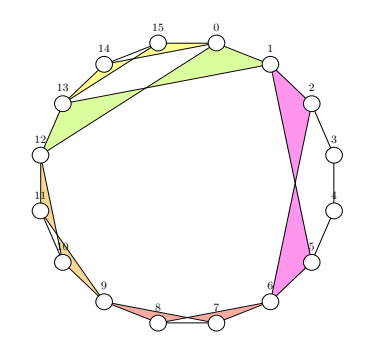
\includegraphics{images/drums.png}
    \caption{A graph $G$ satisfying Properties $1,2,3$, and thus $G \in \mathfrak{H}$. Each drum is shaded in a different colour.}
    \label{fig:Figure-1}
\end{figure}\medskip\\

\textbf{Theorem 1.4.} If $\mu(G) \ne 1$, $\bar\mu(G)=\mu(G)$.\\
The above theorem is from Chandran and Gajjala\cite{chandran_gajjala1000}.\medskip\\
Theorem 1.4 was proved in \cite{chandran_gajjala1000} and thus the structural characterization provided for Type-$2$ graphs was sufficient to find the weighted matching index of Type-$2$ graphs.\\
Chandran and Gajjala also provided an $O(|V||E|)$ algorithm to find whether a given graph is a Type-$2$ graph. \textit{I was able to provide a rough implementation of the algorithm, which is given in Appendix 1.}\medskip\\
\textbf{Corollary.} There exists a graph $G$, such that $\mu(G)=1$ and $\bar\mu(G)=2$.\\
Figure $2$ contains an example of such a graph $G$ such that $\bar\mu(G)=2$ and $\mu(G)=1$. \\
\begin{figure}[h]
    \centering
    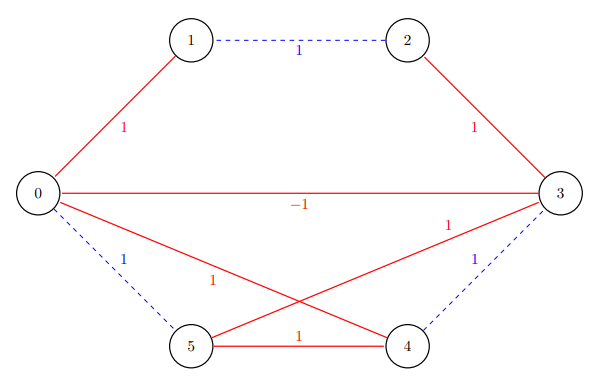
\includegraphics[scale=0.7]{images/mu_different.png}
    \caption{A graph $G$ satisfying $\mu(G)=1$ and $\bar\mu(G)=1$. There is a non-monochromatic perfect matching $M=\{(0,4),(3,5),(1,2)\}$ in $G$, thus $\mu(G)=1$, however, there are no non-monochromatic perfect matchings $M$ such that $w(M) \ne 0$. Thus $\bar\mu(G)=2$.}
    \label{fig:Figure-2}
\end{figure}\medskip\\\\
Theorem 1.4 by Chandran and Gajjala\cite{chandran_gajjala1000} settled Conjecture 1 for Type-$2$ graphs.\\
Additionally, for Type-$1$ graphs, Chandran and Gajjala\cite{cg2023root2} also provided an upper bound: $\bar\mu(G) \le \frac{\displaystyle|V(G)|}{\displaystyle\sqrt{2}}$.
\bigskip\\

\section{Perfect Matchings in Hypergraphs}
\subsection*{Introduction}
Hypergraphs can be visualized as a generalization of graphs, where each edge of a hypergraph can contain multiple vertices. The relatively recent interesting insights provided by the study of monochromatic perfect matchings in graphs thus also motivates understanding the nature of monochromatic perfect matchings in hypergraphs. In this later portion of the report, I state what I studied, understood, and worked on during the last two months about the nature of perfect matchings in $k$-uniform hypergraphs.

\subsection*{Notation and preliminaries}
A \textit{hypergraph} $\mathcal{H}=(V,\mathcal{E})$ is a structure that contains \textit{vertices} or \textit{nodes}, referred to as $V(\mathcal{H})$ and \textit{edges} referred to as $\mathcal{E}(\mathcal{H})$. Unlike a graph, an edge $e \in \mathcal{E}(\mathcal{H})$ can connect any subset $S \subseteq V(\mathcal{H})$ in $\mathcal{H}$.\\
We call a hypergraph $\mathcal{H}$ to be \textit{$k$-uniform} if $\forall$ $e \in \mathcal{E}(\mathcal{H})$, $e$ connects exactly $k$ vertices of $\mathcal{H}$. A simple graph can thus be classified as a $2$-uniform hypergraph.\\
Similar to a graph, a \textit{matching} $M \subseteq \mathcal{E}(\mathcal{H})$ is a subset of edges in $\mathcal{H}$ such that no two edges in a matching share a common vertex. In other words, for any $e_1,e_2 \in M$, $e_1 \ne e_2$, $e_1 \cap e_2=\phi$. A \textit{perfect matching} is a matching which contains all the vertices of $\mathcal{H}$.\\
An edge $e \in \mathcal{E}(\mathcal{H})$ is represented as a subset of vertices of $\mathcal{H}$. We write it as $e=\{v_1,v_2,\dots,v_{k-1},v_k\}$, where $v_1,v_2,\dots,v_k \in V(\mathcal{H})$. In a $k$-uniform hypergraph, $\forall$ $e \in \mathcal{E}(\mathcal{H})$, $|e|=k$. It is easy to see that in a $k$-uniform hypergraph with $n$ vertices, $k | n$.

\subsection*{Monochromatic perfect matchings in hypergraphs}
Let $c$ be a normal edge-colouring of $\mathcal{H}$, and let us represent the normally edge-coloured hypergraph with an edge-colouring $c$ as $\mathcal{H}_c$. Let there be a perfect matching $\mathcal{M}$ of the normally edge-coloured hypergraph $\mathcal{H}_c$. Let $e_v \in \mathcal{M}_c$ be the edge containing the vertex $v \in V(\mathcal{H})$ in $\mathcal{M}_c$. We say a vertex colouring $vc_\mathcal{M}$ to be \textit{induced} by $c$, if $\forall$ $v \in V(\mathcal{H})$, $v$ belongs to the same colour class as $e_v$. We call $\mathcal{M}$ to be a \textit{monochromatic perfect matching} if all vertices of $\mathcal{H}$ are coloured by the same colour class in $vc_\mathcal{M}$.\\
A $n$-uniform hypergraph $\mathcal{H}$ is said to be \textit{perfectly monochromatic} if the following properties hold:
\begin{enumerate}
    % \item $\forall \hspace{0.1cm} e \in E$, $e$ must be part of some perfect matching $\mathcal{M}$.
    \item Every perfect matching, $\mathcal{M}$ of $\mathcal{H}$ is monochromatic.
    \item Let $\mathcal{C}$ be set of colour classes such that $\exists$ a perfect matching $\mathcal{M}$ of $H$ such that $\mathcal{M}$ belongs to a colour class $c \in \mathcal{C}$. Then $\forall \hspace{0.1cm} c \in \mathcal{C}$, $c$ must belong to \textit{exactly} $1$ perfect matching $\mathcal{M}$ of $H$.
\end{enumerate}
Now, for a perfectly monochromatic hypergraph $\mathcal{H}$, we call the dimension $D(\mathcal{H})=|\mathcal{C}|$ of the hypergraph to be the number of colours in it.\\
We are intereseted in finding the bounds on $D(\mathcal{H})$ for a $n$-uniform hypergraph containing $k\cdot n$ vertices.

\subsection*{Results obtained so far}
\textbf{Theorem 2.1.} For a $k$-uniform hypergraph $\mathcal{H}$ with $k$ vertices, $D(\mathcal{H})=1$.\\
\textbf{Proof.} Suppose not. Then $D(\mathcal{H}) \ge 2$. This means that $|\mathcal{E}(\mathcal{H})| \ge 2$, which implies $V(\mathcal{H}) \ge 2 \cdot k$. But $|V(\mathcal{H})|=k$. Contradiction. $\square$ \medskip\\
Krenn claimed \cite{krenn_hypergraph} that for $k$-uniform hypergraphs with $2k$ vertices, where $k=[2,7]$, the number of disjoint perfect matchings corresponds to \cite{oeis1}.\medskip\\
To study the bounds on $D(\mathcal{H})$ $k$-uniform hypergraphs, we start with finding the upper bound on $D(\mathcal{H})$ for $3$-uniform hypergraphs.\\
Let $n=|V(\mathcal{H})|$. We define $\mathcal{D}(\mathcal{H})$ as $D(H)=\max\limits_{\mathcal{H} \in \mathfrak{K}} D(\mathcal{H})$, where $\mathfrak{K}$ refers to all $k$-uniform hypergraphs with $n$ vertices.

\subsection*{Upper bounds on $D(\mathcal{H})$ for $3$-uniform hypergraphs}
\begin{enumerate}
    \item \textit{For a $3$-uniform hypergraph $\mathcal{H}$ with $3$ vertices, $\mathcal{D}(\mathcal{H})=1$.}\\
    From Theorem 2.1, we know that $D(\mathcal{H})$ for a $k$-uniform hypergraph with $k$ vertices is $1$. It directly follows that for a $3$-uniform hypergraph with $3$ vertices, $\mathcal{D}(\mathcal{H})=1$.
    \item \textit{For a $3$-uniform hypergraph $\mathcal{H}$ with $6$ vertices, $\mathcal{D}(\mathcal{H})=10$.}\\
    In a complete $3$-uniform graph with $6$ vertices, $|\mathcal{E}(\mathcal{H})|=\displaystyle\binom{6}{3}=20$. We can colour each edge and its complement with the same colour, forming a monochromatic perfect matching, and thus the number of monochromatic perfect matchings for a $3$-uniform hypergraph with $|V|=6$ is $\frac{20}{2}=10$.
    \item \textit{For a $3$-uniform hypergraph $\mathcal{H}$ with $9$ vertices, $\mathcal{D}(\mathcal{H})=13$.}\\
    This was a known result, however I verified it independently by writing a program which generated $D(\mathcal{H})$ for $3$-uniform graphs with $9$ vertices. The algorithm for the program is provided in Appendix 2.
    \item \textit{For a $3$-uniform hypergraph $\mathcal{H}$ with $12$ vertices, $\mathcal{D}(\mathcal{H})=10$.}\\
    I wrote a partly randomized program, which is provided in Appendix 3, which generated the above result. This suprisingly coincides with $\mathcal{D}(\mathcal{H})$ for a $3$-uniform hypergraph with $6$ vertices.
\end{enumerate}
For calculating the dimensions of $3$-uniform hypergraphs with $9$ and $12$ vertices, we assumed that $\mathcal{H}$ was a complete graph. Now, we first randomly selected any $e \in \mathcal{E}(\mathcal{H})$, and then selected a perfect matching $M$ which contained that edge. This ruled out all edges $e'$ such that $M \cap e' \ne \phi$. We then discarded such edges from our list, and recursively repeated the same process till no matchings could be formed from the remaining list of edges.\medskip\\
We tried using a computational approach for computing $\mathcal{D}(\mathcal{H})$. However, it becomes computationally infeasible to generate $D(\mathcal{H})$ for larger values of $|V(\mathcal{H})|$.\bigskip\\



\bibliographystyle{unsrt}
\bibliography{bibliography}

\bigskip

\section*{Appendix}

\subsection*{1. Implementation of algorithm to decide whether a non-trivial matching covered graph non-isomorphic to $K_4$ is Type-$1$ or Type-$2$ in \cite{chandran_gajjala1000}}\medskip
The file \texttt{max\_matching.py} used to find the maximum matching of a graph using the Edmonds-Blossom algorithm can be found in \cite{edmonds-blossom}.
\subsection*{1.1. Program to check if a graph is connected or not}
\begin{lstlisting}[language=Python]
def dfs(curnode, adj_list, vis):
  vis.add(curnode)
  for e in adj_list[curnode]:
    if e not in vis:
      dfs(e, adj_list, vis)

def check_connected(adj_list, nv):
  vis=set()
  dfs(0, adj_list, vis)
  if len(vis)<nv: return False
  else: return True    
\end{lstlisting}
\subsection*{1.2. Program to convert a graph $G$ to its corresponding matching-covered graph $mcg(G)$}
\begin{lstlisting}[language=Python]
from max_matching import Node, Match

def convert(edges, nv):
  esz=len(edges)
  edges_copy=[]
  already_removed=set()
  for i in range(esz):
    v1, v2=edges[i][0], edges[i][1]
    edges_copy.clear()
    for j in range(esz):
      if j in already_removed: continue
      if edges[j][0]==v1 or edges[j][0]==v2 or edges[j][1]==v1 or edges[j][1]==v2:
        continue
      cv1, cv2=edges[j][0], edges[j][1]

      if v1==nv-2:
        pass
      elif v2==nv-2:
        if cv1==nv-1 and v1<nv-2: cv1=v1
        elif cv2==nv-1 and v1<nv-2: cv2=v1
      else:        
        if cv1==nv-2 and v1<nv-2: cv1=v1
        elif cv2==nv-2 and v1<nv-2: cv2=v1
        if cv1==nv-1 and v2<nv-2: cv1=v2
        elif cv2==nv-1 and v2<nv-2: cv2=v2
      edges_copy.append((cv1, cv2))
      edges_copy.append((cv2, cv1))


    match = Match.from_edges(nv-2, edges_copy)
    unmatched_nodes = match.unmatched_nodes()
    if unmatched_nodes>0:
      already_removed.add(i)

  edges_copy=[]
  for e in edges: edges_copy.append(e)
  for e in already_removed: edges_copy.remove(edges[e])
  return edges_copy


def convert_to_mcg(adj_list, nv):
  edges_here=[]
  for i in range(nv):
    for e in adj_list[i]:
      if e>i:
        edges_here.append([i, e])

  final_edges=convert(edges_here, nv)
  if final_edges:
    print('')
    print('--------------------------------------------------')
    print('Edges in the matching covered graph are:')
    for e in final_edges:
      print('(', e[0]+1, ',', e[1]+1, ')')
    print('--------------------------------------------------\n')

  for i in range(nv):
    for e in adj_list[i]:
      if e>i:
        if [i, e] not in final_edges:
          adj_list[i].remove(e)
          adj_list[e].remove(i)
  return adj_list
\end{lstlisting}

\subsection*{1.3. Program to check whether a matching-covered graph non-isomorphic to $K_4$ is Type-$1$ or Type-$2$}
\begin{lstlisting}[language=Python]
from max_matching import Node, Match
import random
import convert_g_to_mcg
import check_if_connected

def dfs(adjacency_list, visited, curnode, avoid1, avoid2, avoid3):
  if curnode == avoid1 or curnode == avoid2 or curnode == avoid3: return
  visited[curnode] += 1
  for e in adjacency_list[curnode]:
    if e == avoid1 or e == avoid2 or e == avoid3: continue
    if visited[e] > 0: continue
    dfs(adjacency_list, visited, e, avoid1, avoid2, avoid3)


def check_connected(adjacency_list, nv):
  # checking for 2-connectivity
  for i in range(nv):
    for j in range(i+1, nv):
      tdfs = 0
      while tdfs == i or tdfs == j: tdfs += 1
      visited = [0 for i in range(nv)]
      dfs(adjacency_list, visited, tdfs, i, j, -1)
      for k in range(nv):
        if k == i or k == j: continue
        if visited[k] == 0: return 2

  # checking for 3-connectivity
  for i in range(nv):
    for j in range(i+1, nv):
      for k in range(j+1, nv):
        tdfs = 0
        while tdfs == i or tdfs == j or tdfs == k: tdfs += 1
        visited = [0 for i in range(nv)]
        dfs(adjacency_list, visited, tdfs, i, j, k)
        for l in range(nv):
          if l == i or l == j or l == k: continue
          if visited[l] == 0: return 3

  return -1


def find_mu(adjacency_list, degrees, nv):
  v = random.randint(0, nv-1)

  if max(degrees) >= 5: return 1

  all_matchings = []
  for u in adjacency_list[v]:
    nodes = [Node() for i in range(nv-2)]
    prev_value = [i for i in range(nv)]
    imap = {}
    tval = 0
    for e in nodes:
      imap[e.index] = tval
      tval += 1
    for i in range(nv):
      if i == u or i == v: continue
      curno = i
      if i > u: curno -= 1
      if i > v: curno -= 1
      prev_value[curno] = i
    for i in range(nv):
      if i == u or i == v: continue
      curnode = i
      if i > u: curnode -= 1
      if i > v: curnode -= 1
      for e in adjacency_list[i]:
        neighnode = e
        if e == u or e == v: continue
        if e > u: neighnode -= 1
        if e > v: neighnode -= 1
        nodes[curnode].neighbors.append(nodes[neighnode])
    
    match = Match(nodes)
    un = match.unmatched_nodes()

    already_present = set()
    current_matching = [[min(u,v),max(u,v)]]
    for node in nodes:
      if node.mate != None:
        assert node.mate.mate == node
        num1 = imap.get(node.index)
        num2 = imap.get(node.mate.index)

        if prev_value[num1] in already_present: continue
        smaller, bigger = prev_value[num1], prev_value[num2]
        if smaller > bigger: smaller, bigger = bigger, smaller
        current_matching.append([smaller, bigger])
        already_present.add(prev_value[num1])
        already_present.add(prev_value[num2])

    all_matchings.append(current_matching)

  tot_matchings = len(all_matchings)

  hamiltonian_cycle = []
  w1, w2 = [-1 for i in range(nv)], [-1 for i in range(nv)]

  for i in range(tot_matchings):
    if hamiltonian_cycle: break
    for j in range(i+1, tot_matchings):
      m1, m2 = all_matchings[i], all_matchings[j]
      assert(len(m1) == len(m2) and len(m1) == nv//2)
      is_hamiltonian = True

      for k in range(nv//2):
        if m2[k] in m1:
          is_hamiltonian = False
          break
      if not is_hamiltonian: continue

      ''' checking whether it is only 1 hamiltonian cycle or multiple hamiltonian cycles'''
      all_here = []
      for e in m1: all_here.append(e)
      for e in m2: all_here.append(e)
      all_here.sort()
      count_vertices = {}
      for k in range(nv):
        count_vertices[all_here[k][0]] = count_vertices.get(all_here[k][0], 0) + 1
        count_vertices[all_here[k][1]] = count_vertices.get(all_here[k][1], 0) + 1
        if max(count_vertices.values()) == 2 and min(count_vertices.values()) == 2 and k != nv-1:
          is_hamiltonian = False
          break
      if not is_hamiltonian: continue

      for e in m1:
        w1[e[0]], w1[e[1]] = e[1], e[0]
        hamiltonian_cycle.append(e)
      for e in m2:
        w2[e[0]], w2[e[1]] = e[1], e[0]
        hamiltonian_cycle.append(e)
      break
  
  if not hamiltonian_cycle:
    return 1
  
  re_numbering = [-1 for i in range(nv)]
  re_numbering[0] = 0
  current_number = 1
  current_vertex = w1[0]
  while current_vertex != 0:
    re_numbering[current_vertex] = current_number
    current_number += 1
    if current_number % 2 == 0:
      current_vertex = w2[current_vertex]
    else:
      current_vertex = w1[current_vertex]
  print('=================================================')
  print('Re-numbering of vertices:')
  print('=================================================')
  for i in range(nv):
    print('Original numbering:', i+1, 'Re-numbering:', re_numbering[i])
  print('=================================================\n')

  edge_set = []
  '''checking property 1'''
  for i in range(nv):
    for u in adjacency_list[i]:
      if u > i: continue
      edge_set.append([u, i])
      found = False
      for e in hamiltonian_cycle:
        if (e[0] == i and e[1] == u) or (e[0] == u and e[1] == i):
          found = True
          break
      if not found:
        if re_numbering[u]%2 != re_numbering[i]%2: return 1

  '''checking property 2'''
  n_es = len(edge_set)
  drum_no = [-1 for i in range(n_es)]
  drums = 0
  for i in range(n_es):
    if edge_set[i] in hamiltonian_cycle:
      drum_no[i] = -2
      continue
    if [edge_set[i][1],edge_set[i][0]] in hamiltonian_cycle:
      drum_no[i] = -2
      continue
    for j in range(i+1, n_es):
      if edge_set[i][0] == edge_set[j][1] and edge_set[i][1] == edge_set[j][0]: continue
      e1, e2 = edge_set[i], edge_set[j]
      if e2 in hamiltonian_cycle: continue
      if [edge_set[j][1],edge_set[j][0]] in hamiltonian_cycle: continue


      v1, v2, v3, v4 = re_numbering[e1[0]], re_numbering[e1[1]], re_numbering[e2[0]], re_numbering[e2[1]]
      lv = [v1, v2, v3, v4]
      lv.sort()
      if not((lv[0] == v1 and lv[2] == v2) or (lv[0] == v2 and lv[2] == v1) or (lv[1] == v1 and lv[3] == v2) or (lv[1] == v2 and lv[3] == v1)):
        continue
      
      dec = 0
      is_drum = True
      for k in range(4):
        if lv[k] < lv[k-1]: dec += 1
        if lv[k]%2 != lv[k-2]%2:
          is_drum = False
          break
      if not is_drum or dec != 1: return 1
      def is_adj_vertex(x,y): return abs(x-y) == 1 or abs(x-y) == nv-1
      if (is_adj_vertex(lv[0],lv[1]) and is_adj_vertex(lv[2],lv[3])) or (is_adj_vertex(lv[0],lv[3]) and is_adj_vertex(lv[1],lv[2])):
        if drum_no[i] != -1 or drum_no[j] != -1:
          return 1
        drums += 1
        drum_no[i], drum_no[j] = drums, drums
      else:
        return 1

  '''checking property 3'''
  if -1 in drum_no: return 1
  if max(drum_no) == -2 and min(drum_no) == -2: return 2
  d_count = [0 for i in range(drums)]
  for i in range(n_es):
    if drum_no[i] == -1: return 1
    if drum_no[i] == -2: continue
    d_count[drum_no[i]-1] += 1
  if max(d_count) == 2 and min(d_count) == 2: return 2
  else: return 1

def main():
  nv, ne = 0, 0
  print('Number of vertices in the graph:')
  nv = int(input())
  adj_list = [[] for i in range(nv)]
  degree = [0 for i in range(nv)]
  print('Number of edges in the graph:')
  ne = int(input())
  capacity = [[0 for i in range(nv)] for j in range(nv)]
  print('Edges of the graph (1-indexed):')
  for i in range(ne):
    u, v = map(int, input().split())
    u -= 1
    v -= 1
    adj_list[u].append(v)
    adj_list[v].append(u)   
    degree[u] += 1
    degree[v] += 1
    capacity[u][v] = 1
    capacity[v][u] = 1
  is_graph_connected=check_if_connected.check_connected(adj_list, nv)
  if not is_graph_connected:
    print('Graph is not connected')
    exit(0)
  adj_list=convert_g_to_mcg.convert_to_mcg(adj_list, nv)
  is_graph_connected=check_if_connected.check_connected(adj_list, nv)
  if not is_graph_connected:
    print('Matching covered graph is not connected')
    exit(0)
  connectivity = check_connected(adj_list, nv)
  is_2_connected = (connectivity == 2)
  is_3_connected = (connectivity == 3)


  print('---------------------------------------------------------')
  print('Is 2-connected:', 'Yes' if is_2_connected else 'No')
  print('Is 3-connected:', 'Yes' if is_3_connected else 'No')
  print('---------------------------------------------------------')
  print('')
  print('')
  is_type2 = (find_mu(adj_list, degree, nv) == 2)
  print('===========================================')
  print('Is type 2:', 'Yes' if is_type2 else 'No')
  print('===========================================')

main()
\end{lstlisting}

\subsection*{1.4. Some sample testcases for the code in 1.3}
\begin{lstlisting}
Case 1:

Input-

Number of vertices in the graph:
4
Number of edges in the graph:
4
Edges of the graph (1-indexed):
1 2
2 4
4 3
3 1

Output-

--------------------------------------------------
Edges in the matching covered graph are:
( 1 , 2 )
( 1 , 3 )
( 2 , 4 )
( 3 , 4 )
--------------------------------------------------

---------------------------------------------------------
Is 2-connected: Yes
Is 3-connected: No
---------------------------------------------------------


=================================================
Re-numbering of vertices:
=================================================
Original numbering: 1 Re-numbering: 0
Original numbering: 2 Re-numbering: 3
Original numbering: 3 Re-numbering: 1
Original numbering: 4 Re-numbering: 2
=================================================

===========================================
Is type 2: Yes
===========================================


Case 2:

Input-

Number of vertices in the graph:
6
Number of edges in the graph:
6
Edges of the graph (1-indexed):
1 4
4 2
2 3
3 6
6 5
5 1

Output-

--------------------------------------------------
Edges in the matching covered graph are:
( 1 , 4 )
( 1 , 5 )
( 2 , 4 )
( 2 , 3 )
( 3 , 6 )
( 5 , 6 )
--------------------------------------------------

---------------------------------------------------------
Is 2-connected: Yes
Is 3-connected: No
---------------------------------------------------------


=================================================
Re-numbering of vertices:
=================================================
Original numbering: 1 Re-numbering: 0
Original numbering: 2 Re-numbering: 4
Original numbering: 3 Re-numbering: 3
Original numbering: 4 Re-numbering: 5
Original numbering: 5 Re-numbering: 1
Original numbering: 6 Re-numbering: 2
=================================================

===========================================
Is type 2: Yes
===========================================
\end{lstlisting}


\subsection*{2.1. Code for generating $D(\mathcal{H})$ for $|V(\mathcal{H})|=9$}
\begin{lstlisting}[language=C++]
#include <bits/stdc++.h>
#include "C:\Users\DARPAN\Documents\CP\debugger.h"
using namespace std;

const int N = 9;

vector<vector<vector<int>>> solve() {
  /* Brute force idea:
   * Select an arbitrary tuple (u, v, w).
   * Now for that arbitrary tuple, check how many edges cannot form edges anymore, in other words
   * strike out the invalid edges.
   * Randomly shuffle and see how that goes. */

  /* Generate all NC3 possible tuples first */
  vector<vector<int>> tuples;
  for (int i = 1; i <= N; i++) {
    for (int j = i + 1; j <= N; j++) {
      for (int k = j + 1; k <= N; k++) {
        tuples.push_back(vector<int>{i, j, k});
      }
    }
  }
  mt19937 rng(chrono::steady_clock::now().time_since_epoch().count()); /* random generator */
  shuffle(tuples.begin(), tuples.end(), rng);

  vector<vector<vector<int>>> taken;
  set<vector<int>> invalid;
  for (int i = 0; i < (int)tuples.size(); i++) {
    vector<vector<int>> cur_tuple;
    if (invalid.find(tuples[i]) != invalid.end()) continue;
    cur_tuple.push_back(tuples[i]);
    for (int j = 0; j < (int)tuples.size(); j++) {
      if (j == i) continue;
      if (invalid.find(tuples[j]) != invalid.end()) continue;
      cur_tuple.push_back(tuples[j]);
      set<int> left;
      for (int k = 1; k <= N; k++) left.insert(k);
      for (auto e : cur_tuple) for (auto f : e) left.erase(f);
      if (left.size() != 3) {
        cur_tuple = {tuples[i]};
        continue;
      }
      vector<int> last_tuple;
      for (auto e : left) last_tuple.push_back(e);
      if (invalid.find(last_tuple) != invalid.end()) {
        cur_tuple.pop_back();
        continue;
      }
      cur_tuple.push_back(last_tuple);

      /* if even 1 edge is common, then it is invalid */
      auto is_valid = [&]() {
        for (auto e : taken) {
          for (auto f : e) {
            for (auto g : cur_tuple) {
              if (f[0] == g[0] && f[1] == g[1] && f[2] == g[2]) {
                return false;
              }
            }
          }
        }
        for (auto e : cur_tuple) {
          if (invalid.find(e) != invalid.end()) {
            return false;
          }
        }
        return true;
      };

      if (is_valid()) {
        for (auto e : taken) {
          for (auto f : e) {
            set<int> left2;
            for (auto g : cur_tuple) {
              for (int i = 1; i <= N; i++) left2.insert(i);
              for (auto h : g) left2.erase(h);
              for (auto h : f) left2.erase(h);
              vector<int> ltuple;
              for (auto h : left2) ltuple.push_back(h);
              if (ltuple.size() == 3) invalid.insert(ltuple);
            }
          }
        }
        sort(cur_tuple.begin(), cur_tuple.end());
        taken.push_back(cur_tuple);
        break;
      } else {
        cur_tuple = {tuples[i]};
      }
    }
  }

  sort(taken.begin(), taken.end());
  for (auto e : taken) for (auto f : e) {
    if (invalid.find(f) != invalid.end()) {
      assert(false);
    } 
  }
  return taken;
}

int main() {
  for (int i = 0; i < 1000; i++) {
    auto taken = solve();
    
    /* printing the matchings */
    if (taken.size() >= 13) {
      cout << "TOTAL MATCHINGS = " << taken.size() << '\n';
      for (auto e : taken) {
        for (auto f : e) {
          cout << '{' << f[0] << ", " << f[1] << ", " << f[2] << "}, "; 
        }
        cout << '\n';
      }
      cout << '\n';
    }
  }
  return 0;
}

\end{lstlisting}

\subsection*{2.2. Example of $D(\mathcal{H})=13$ produced by the above code}
\begin{lstlisting}
TOTAL MATCHINGS = 13
{1, 2, 3}, {4, 6, 8}, {5, 7, 9},
{1, 2, 4}, {3, 5, 6}, {7, 8, 9},
{1, 2, 5}, {3, 6, 7}, {4, 8, 9},
{1, 2, 8}, {3, 5, 7}, {4, 6, 9},
{1, 3, 4}, {2, 7, 9}, {5, 6, 8},
{1, 3, 9}, {2, 6, 7}, {4, 5, 8},
{1, 4, 7}, {2, 6, 9}, {3, 5, 8}, 
{1, 5, 6}, {2, 7, 8}, {3, 4, 9},
{1, 5, 9}, {2, 3, 6}, {4, 7, 8},
{1, 6, 7}, {2, 4, 5}, {3, 8, 9},
{1, 6, 8}, {2, 5, 9}, {3, 4, 7},
{1, 6, 9}, {2, 3, 8}, {4, 5, 7},
{1, 7, 8}, {2, 4, 6}, {3, 5, 9},
\end{lstlisting}


\subsection*{3.1. Code for generating $D(\mathcal{H})$ for $|V(\mathcal{H})|=12$}
\begin{lstlisting}[language=C++]
#include <bits/stdc++.h>
#include "C:\Users\DARPAN\Documents\CP\debugger.h"
using namespace std;

const int N = 12;

vector<vector<vector<int>>> find_mu() {
  vector<vector<vector<int>>> matchings;
  set<pair<vector<int>, vector<int>>> forbidden;
  set<vector<int>> added;
  vector<vector<int>> tuples;
  for (int i = 1; i <= N; i++) {
    for (int j = i + 1; j <= N; j++) {
      for (int k = j + 1; k <= N; k++) {
        tuples.push_back({i, j, k});
      }
    }
  }
  mt19937 rng(chrono::steady_clock::now().time_since_epoch().count());
  shuffle(tuples.begin(), tuples.end(), rng);
  int n_tuples = tuples.size();
  for (int i = 0; i < n_tuples; i++) {
    vector<vector<int>> cur_matching;
    for (int j = i; j < n_tuples; j++) {
      if (cur_matching.size() == 4)
        break;
      bool is_ok = true;
      if (added.count(tuples[j]))
        continue;
      for (auto e : cur_matching) {
        for (auto f : e) {
          for (auto g : tuples[j]) {
            if (f == g) {
              is_ok = false;
              break;
            }
          }
        }
      }
      if (!is_ok)
        continue;
      for (auto e : added) {
        if (forbidden.count(make_pair(e, tuples[j])) || forbidden.count(make_pair(tuples[j], e))) {
          is_ok = false;
          break;
        }
      }
      if (!is_ok)
        continue;
      for (auto e : added) {
        for (auto f : added) {
          for (auto g : added) {
            set<int> all;
            for (auto h : e)
              all.insert(h);
            for (auto h : f)
              all.insert(h);
            for (auto h : g)
              all.insert(h);
            for (auto h : tuples[j])
              all.insert(h);
            if (all.size() == 12) {
              is_ok = false;
              break;
            }
          }
        }
      }
      if (!is_ok)
        continue;
      for (auto e : added){
        for (auto f : added) {
          for (auto g : cur_matching) {
            set<int> all;
            for (auto h : e)
              all.insert(h);
            for (auto h : f)
              all.insert(h);
            for (auto h : g)
              all.insert(h);
            for (auto h : tuples[j])
              all.insert(h);
            if (all.size() == 12) {
              is_ok = false;
              break;
            }
          }
        }
      }
      if (!is_ok)
        continue;
      for (auto e : added) {
        for (auto f : cur_matching) {
          for (auto g : cur_matching) {
            set<int> all;
            for (auto h : e)
              all.insert(h);
            for (auto h : f)
              all.insert(h);
            for (auto h : g)
              all.insert(h);
            for (auto h : tuples[j])
              all.insert(h);
            if (all.size() == 12) {
              is_ok = false;
              break;
            }
          }
        }
      }
      if (!is_ok)
        continue;
      cur_matching.push_back(tuples[j]);
    }
    if (cur_matching.size() != 4)
      continue;
    sort(cur_matching.begin(), cur_matching.end());
    matchings.push_back(cur_matching);
    for (auto e : cur_matching)
      added.insert(e);
    for (int j = 0; j < 4; j++) {
      for (int k = j + 1; k < 4; k++) {
        set<int> all;
        for (int l = 1; l <= N; l++)
          all.insert(l);
        for (auto e : cur_matching[j])
          all.erase(e);
        for (auto e : cur_matching[k])
          all.erase(e);
        assert(all.size() == 6);
        vector<int> rest;
        for (auto e : all)
          rest.push_back(e);
        do {
          vector<int> v1, v2;
          for (int l = 1; l < 3; l++)
            v1.push_back(rest[l]);
          for (int l = 3; l <= 5; l++)
            v2.push_back(rest[l]);
          forbidden.insert(make_pair(v1, v2));
        } while (next_permutation(rest.begin(), rest.end()));
      }
    }
  }
  sort(matchings.begin(), matchings.end());
  return matchings;
}
\end{lstlisting}

\subsection*{3.2. Example of $D(\mathcal{H})=10$ produced by the above code}
\begin{lstlisting}
10
{1, 2, 6, }, {3, 5, 10, }, {4, 8, 9, }, {7, 11, 12, },
{1, 2, 12, }, {3, 9, 10, }, {4, 6, 8, }, {5, 7, 11, },
{1, 3, 4, }, {2, 6, 10, }, {5, 9, 11, }, {7, 8, 12, }, 
{1, 3, 9, }, {2, 4, 10, }, {5, 8, 11, }, {6, 7, 12, },
{1, 3, 11, }, {2, 5, 9, }, {4, 10, 12, }, {6, 7, 8, },
{1, 4, 7, }, {2, 3, 5, }, {6, 8, 11, }, {9, 10, 12, },
{1, 5, 8, }, {2, 7, 10, }, {3, 11, 12, }, {4, 6, 9, },
{1, 5, 12, }, {2, 3, 8, }, {4, 7, 10, }, {6, 9, 11, },
{1, 7, 12, }, {2, 8, 9, }, {3, 5, 6, }, {4, 10, 11, },
{1, 8, 11, }, {2, 4, 12, }, {3, 5, 7, }, {6, 9, 10, },
\end{lstlisting}

\section*{Acknowledgement}
I would like to thank the \textit{IASc-INSA-NASI} for providing such a wonderful opportunity and {Prof. L. Sunil Chandran}, Department of CSA, IISc Bengaluru for mentoring me during the summer fellowship.\\
I would also like to thank PhD scholars and postdoctoral researchers under Prof. Chandran for helping and guiding me during the fellowship.\\

\end{document}
